\documentclass[12pt]{article}

\usepackage[margin=0.8in]{geometry}
\usepackage{graphicx}
\usepackage{float}
\usepackage{setspace}
\singlespacing
\usepackage{booktabs}
\usepackage[dvipsnames]{xcolor}
\usepackage{comment}
\usepackage{setspace}
\usepackage{amsmath}
\usepackage{xcolor}
\usepackage{chngcntr}
\usepackage{caption}
\usepackage{hhline}
\usepackage{hyperref}
\usepackage{multirow}
\usepackage{rotating}
\usepackage{subcaption}
\usepackage{longtable}
\usepackage{placeins}
\usepackage{amsmath}
\usepackage{amssymb}
\usepackage{tikz, pgfplots}
\usepackage{hyperref}
% \usepackage{minipage}

\newcommand{\tick}{\checkmark}

\title{Convolutions for Causal Panel Data Models:\\
	An Application to California's Proposition 99 Data
}
\author{
	Wooyong Park\\
	\multicolumn{1}{p{.7\textwidth}}{\centering Yonsei University} 
}

\date{Deep Learning(STA 3140) Final Project}

\renewcommand{\abstractname}{Abstract}

\hypersetup{
	colorlinks=true,    
	citecolor=blue,     
	filecolor=magenta,   
	urlcolor=cyan          
}
\captionsetup[table]{name=Table}
\captionsetup[figure]{name=Figure}

\usepackage[backend=biber, style=authoryear, maxcitenames=2, maxbibnames=9]{biblatex}
\renewbibmacro{in:}{}
\DeclareDelimFormat{nameyeardelim}{\addcomma\space}
\addbibresource{bibliography.bib}



\begin{document}
	\begin{singlespace}
		\maketitle
	\end{singlespace}
	
	\begin{figure}[htbp]
		\centering
		\begin{subfigure}[c]{0.3\textwidth}
			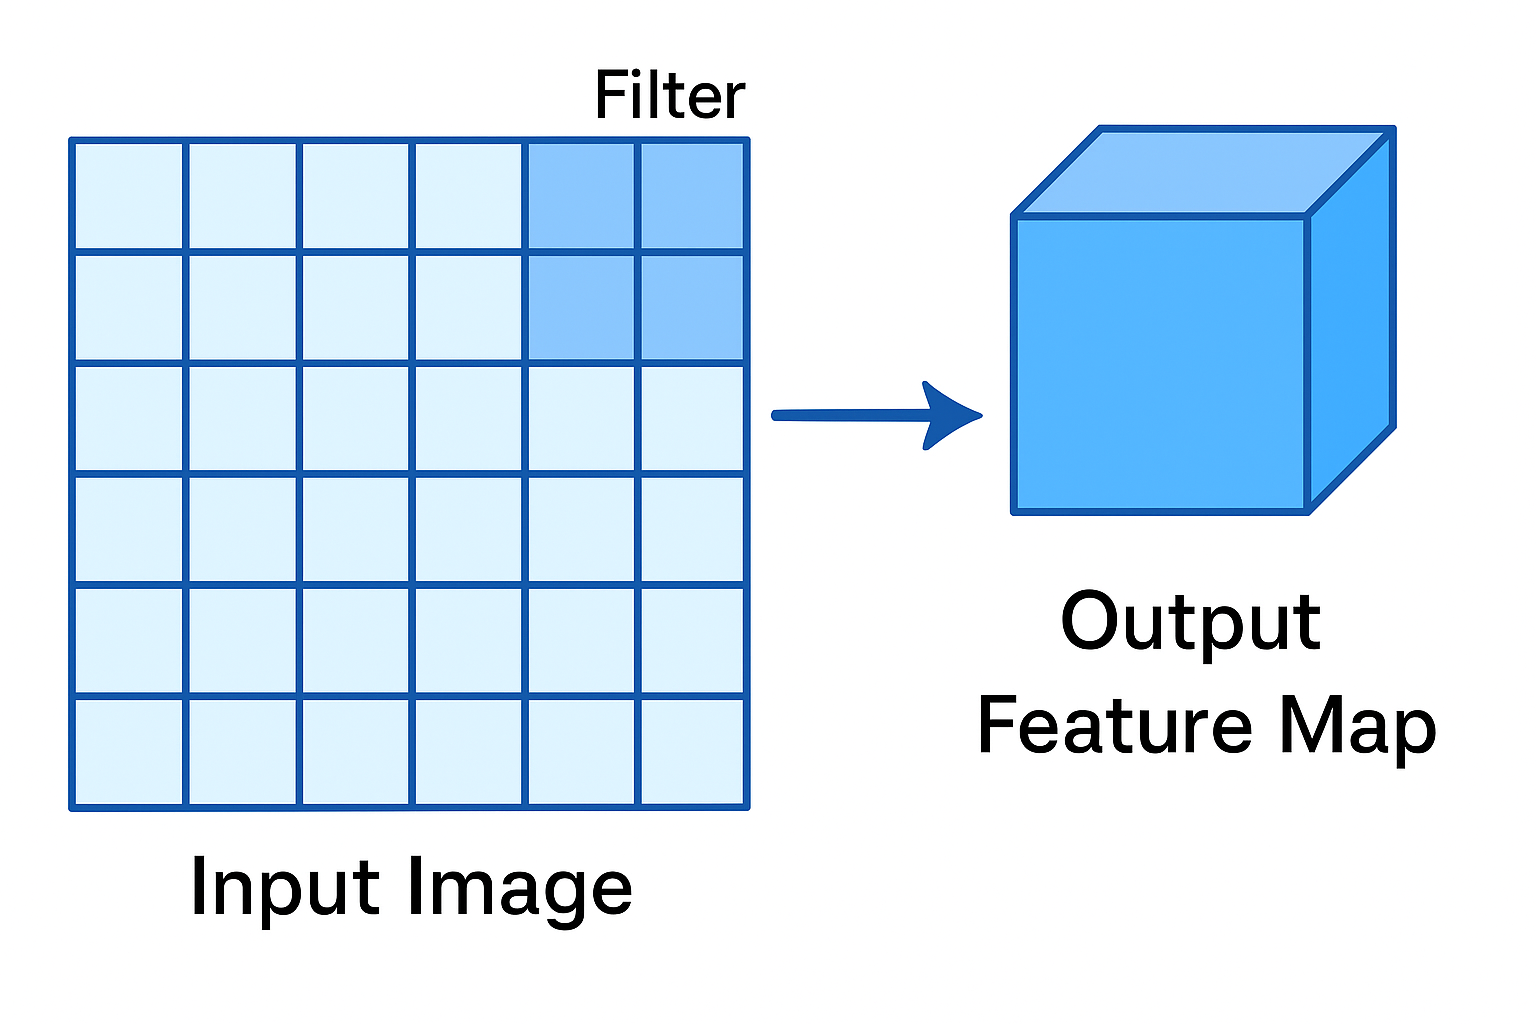
\includegraphics[width=\textwidth]{../figures/intro1.png}
		\end{subfigure}
		\hspace{10pt}
		{\Large $\Longrightarrow$}
		\hspace{10pt}
		\begin{subfigure}[c]{0.3\textwidth}
			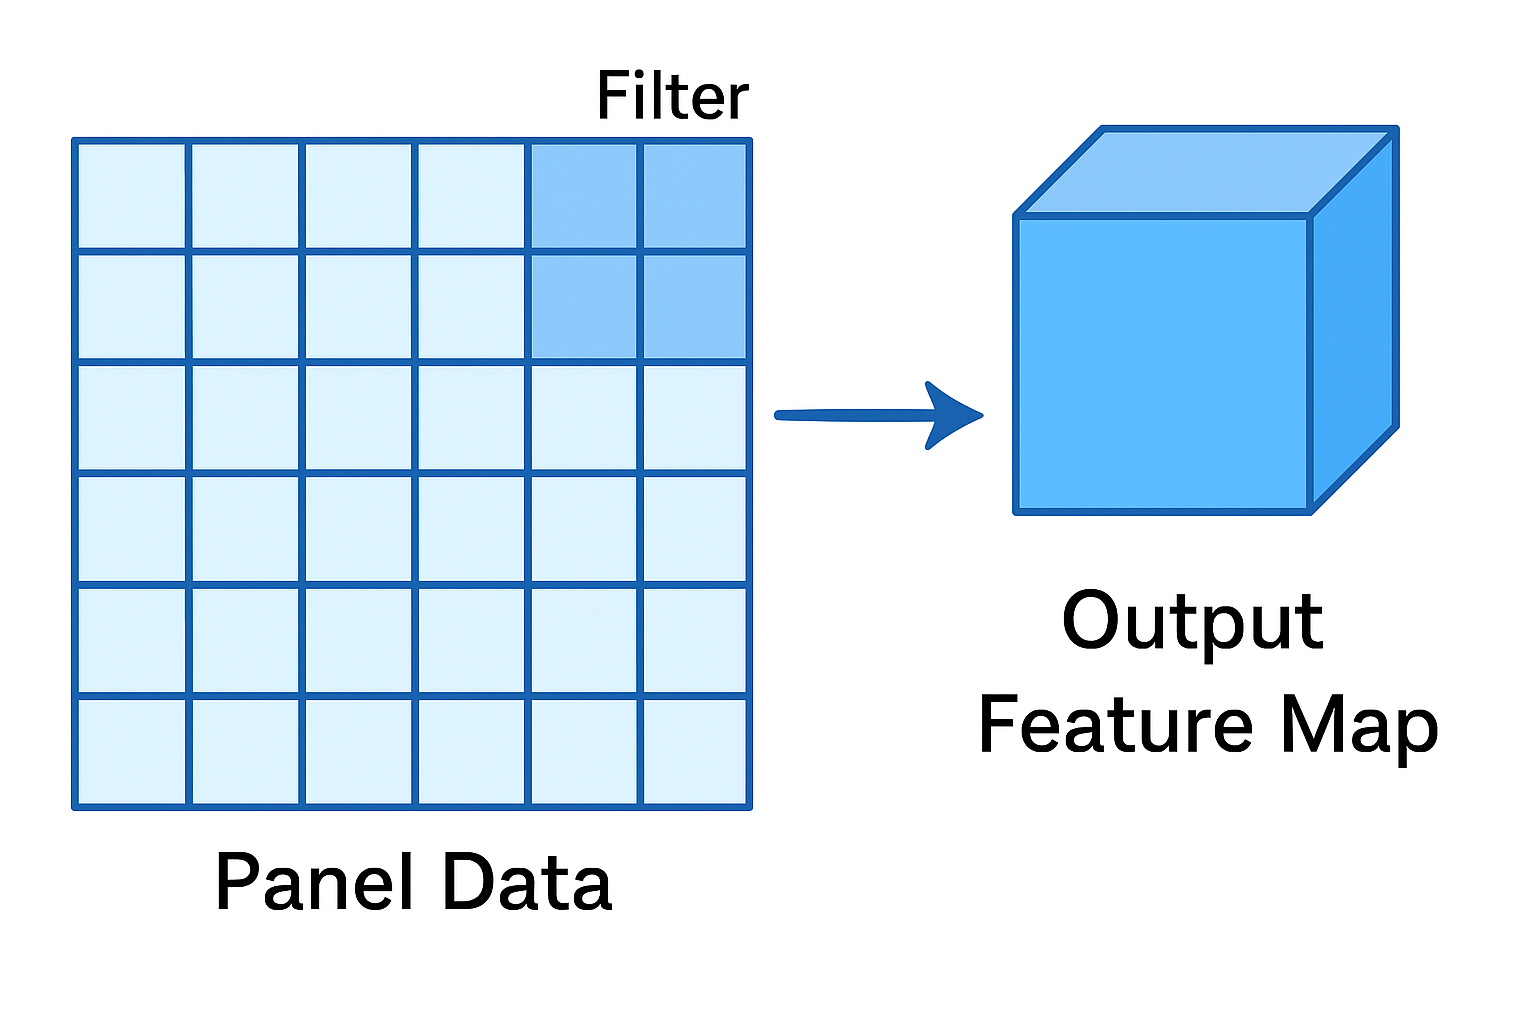
\includegraphics[width=\textwidth]{../figures/intro2.png}
		\end{subfigure}
	\end{figure}
	\begin{abstract}		
		\begin{singlespace} 
			This study explores the possibility of applying convolutional neural networks (CNNs) to panel data, particulary in the context of causal inference.
			CNNs have shown remarkable performance in image recognition tasks, but their application to panel data analysis is still limited.
			On the contrary, traditional econometric methods, such as fixed effects, difference-in-differences, and synthetic control, have been widely used for causal inference in panel data.
			However, these methods often rely on strong assumptions and may not be suitable for complex data structures.
			To address this issue, we propose a novel approach that combines CNNs and Mahalanobis covariate distance to estimate causal effects in panel data.
			We demonstrate the effectiveness of our approach using California's Proposition 99 data, which examines the impact of tobacco control policies on smoking rates and
			compare the results with those obtained from Matrix Completion (MC-NNM) methods.
		\end{singlespace}
		
		\bigskip
		\noindent \emph{Keywords: Policy Evaluation, Matrix Completion, Convolutional Neural Networks, Panel Data}
		\vspace{0.2cm}

		\noindent \emph{Codes and Figures: \href{https://github.com/wooyongp/deep-learning-final}{Github Repo}}
		\vspace{0.2cm}

		\noindent \emph{Data: Click \href{https://drive.google.com/uc?id=1wD8h8pjCLDy1RbuPDZBSa3zH45TZL7ha&export=download}{this link}}
		
		
		% \vfill
		
		% \centering
		% We thank those who provided valuable comments on this study.
		
	\end{abstract}		

\newpage

\fontsize{11pt}{11pt}\selectfont
\section{Introduction}


Estimating treatment effects of policy interventions in panel data is a challenging task due to the presence of unobserved counterfactuals and the need for robust estimation methods.
Traditional econometric methods have been widely used for their ability to model these counterfactuals and provide reliable estimates and confidence intervals under paticular assumptions, most closely based on the potential outcomes framework of \textcite{rubin1974estimating}.
However, these methods often implicitly or explicitly assume parametric forms of the data generating process, such as linearity or normality, which may not hold in practice.

This study explores the possibility of applying convolutional neural networks (CNNs) to panel data, particularly in the context of causal inference.
Multiple studies have used nontraditional methods 
or machine learning methods to estimate treatment effects in panel data.
For example, \textcite{athey2021matrix} have proposed a matrix completion method with nuclear norm regularization (MC-NNM henceforth) to estimate treatment effects in panel data that relies on cross validation to choose the
right degree of regularization.
Also, \textcite{abadie2010synthetic} have proposed a synthetic control method that uses 
a weighted average of control units to construct a counterfactual for the treated unit.
A natural extension to these methods is to use neural networks, which have shown remarkable performance in prediction tasks of high-dimensional data, such as images and text.


The main task of this study is to predict the counterfactual outcomes of a treated unit in a panel data setting with CNN, denoted 
as $\mathbf{Y(0)}$ in equation \eqref{eq:panel_data_Y0}.
Each row of $\mathbf{Y(0)}$ represents the sequence of outcomes of a unit, and the columns represent different time periods.
The treated unit is in the first row, and the red ${\color{red} ?}$'s are the missing counterfactuals we want to predict, as the treated unit's $Y(0)$'s are not observed after the treatment.
The other rows are the outcomes of control units, which are observed for all time periods.

\begin{align}
    	\mathbf{Y(0)}&=\begin{pmatrix}
		\tick  & \tick & {\color{red} ?}   & \dots & {\color{red} ?}  & \leftarrow{\text{treated unit}}\\
		\vdots   &  \vdots & \vdots &\ddots &\vdots& \\
        \tick & \tick & \tick  & \dots & \tick& \\
		\tick  & \tick & \tick   & \dots & \tick & \\
		\tick & \tick & \tick   & \dots & \tick & \\
		\tick & \tick & \tick   & \dots & \tick & 
		\end{pmatrix} 
        \label{eq:panel_data_Y0}
\end{align}


\section{CNNs for Panel Data}


\subsection{Combining CNNs and Mahalanobis Distance}

However, applying CNNs to panel data is not as straightforward as applying them to images.
In images, the input is a 2D matrix of pixel values, and applying convolution operations are reasonable
because nearby pixels are likely to be correlated to each other.
In panel data, although the input is also a 2D matrix, the rows represent different units and the columns represent different time periods.
The correlation between different periods of the same unit is necessarily strong, but the correlation between adjacent units is not necessarily strong.
Put more simply, although the horizontal neighbors of each cell in $\mathbf{Y(0)}$ are likely to be correlated, the vertical neighbors are not.
Therefore, applying CNN to panel data requires modifying $\mathbf{Y(0)}$ so that vertically adjacent cells are also correlated.

To tackle the aforementioned issue, we propose a novel approach that combines CNNs and Mahalanobis covariate distance to estimate causal effects in panel data.
The Mahalanobis distance is a measure of the distance between a point and a distribution, which takes into account the covariance structure of the data:

\begin{align}
    d_{\text{Mahalanobis}}(\mathbf{x}, \mathbf{y}) &= \sqrt{(\mathbf{x} - \mathbf{y})^\top \Sigma^{-1} (\mathbf{x} - \mathbf{y})} \label{eq:mahalanobis_distance}\\
    \text{where } \Sigma &= \text{cov}(\mathbf{x}, \mathbf{y}) \text{ is the covariance matrix of } \mathbf{x} \text{ and } \mathbf{y}. \notag
\end{align}

We compute \eqref{eq:mahalanobis_distance} between the treated unit and each control unit before the treatment, 
and use this Mahalanobis distance to order the control units vertically in $\mathbf{Y(0)}$.
This way, the vertically adjacent cells in $\mathbf{Y(0)}$ are more likely to be correlated, and applying CNNs to $\mathbf{Y(0)}$ is more reasonable:

\begin{align}
        \mathbf{Y(0)}&=\begin{pmatrix}
        \tick  & \tick & {\color{red} ?}   & \dots & {\color{red} ?}  &\\
        \vdots   &  \vdots & \vdots &\ddots &\vdots& \\
        \tick & \tick & \tick  & \dots & \tick& \\
        \tick  & \tick & \tick   & \dots & \tick & \\
        \tick & \tick & \tick   & \dots & \tick & \\
        \tick & \tick & \tick   & \dots & \tick & 
        \end{pmatrix} 
        \quad
        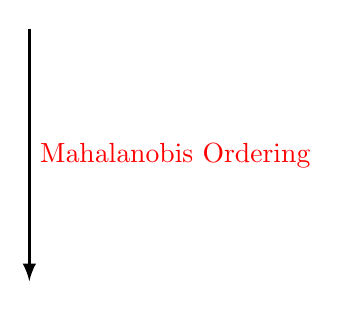
\begin{tikzpicture}[baseline={(current bounding box.center)}]
            \draw[very thick,->,>=latex] (0,1.6) -- (0,-1.6) node[midway,right] {\textcolor{red}{Mahalanobis Ordering}};
        \end{tikzpicture}
\end{align}


\subsection{CNN Configuration}
As opposed to images, the input of CNNs for panel data illustrated in \eqref{eq:panel_data_Y0} is a small matrix of outcomes, 
and thus a complex CNN architecture with too many parameters may lead to overfitting.
Thus, we use a simple CNN architecture with only two convolutional layers: the first layer has 32 filters of size 3$\times$3 with ReLU activation,
and the second layer has one filter of size 3$\times$3 with linear activation.
Both layers use a stride of 1 and zero padding to maintain the input size.
The output of the second layer is a $N \times T$ matrix, where $N$ is the number of units and $T$ is the number of time periods (i.e., the same size as $\mathbf{Y(0)}$).
The CNN is trained to minimize the mean squared error between the predicted outcomes and the actual outcomes of the control units ove all time periods,
and the optimization is performed using the Adam optimizer.

\section{Data}
We use the California Proposition 99 data from \textcite{abadie2010synthetic}, which is a panel data set that contains information on smoking rates and tobacco control policies in California.\footnote{The
data is available at \url{"https://drive.google.com/uc?id=1wD8h8pjCLDy1RbuPDZBSa3zH45TZL7ha&export=download"}.}
 - Table \ref{tab:summary_statistics} presents the summary statistics of the data:

\begin{table}[htbp]
    \centering
    \begin{tabular}{lrrrrrrrr}
\toprule
 & count & mean & std & min & 25\% & 50\% & 75\% & max \\
\midrule
state & 1209.00 & 20.00 & 11.26 & 1.00 & 10.00 & 20.00 & 30.00 & 39.00 \\
year & 1209.00 & 1985.00 & 8.95 & 1970.00 & 1977.00 & 1985.00 & 1993.00 & 2000.00 \\
cigsale & 1209.00 & 118.89 & 32.77 & 40.70 & 100.90 & 116.30 & 130.50 & 296.20 \\
lnincome & 1014.00 & 9.86 & 0.17 & 9.40 & 9.74 & 9.86 & 9.97 & 10.49 \\
beer & 546.00 & 23.43 & 4.22 & 2.50 & 20.90 & 23.30 & 25.10 & 40.40 \\
age15to24 & 819.00 & 0.18 & 0.02 & 0.13 & 0.17 & 0.18 & 0.19 & 0.20 \\
retprice & 1209.00 & 108.34 & 64.38 & 27.30 & 50.00 & 95.50 & 158.40 & 351.20 \\
\bottomrule
\end{tabular}

    \caption{Summary Statistics of the California Proposition 99 Data}
    \label{tab:summary_statistics}
\end{table}


The goal of \textcite{abadie2010synthetic} was to estimate the effect of increased cigarette taxes on cigarette sales in California, which is our goal as well with using CNN. 
The panel contains data from 39 states (including California) from 1970 through 2000.
 California passed Proposition 99 increasing cigarette taxes from 1989 onwards. Thus, we have 1 treated group (California) - with increased cigarette taxes - and 38 states of control group; 19 pre-treatment periods (1970-1988) and 12 post-treatment periods (1989-2000).

 

\section{Results}
\subsection{CNN Results and Comparison with MC-NNM}

\begin{figure}[htbp]
    \centering
        \begin{subfigure}[c]{0.45\textwidth}
        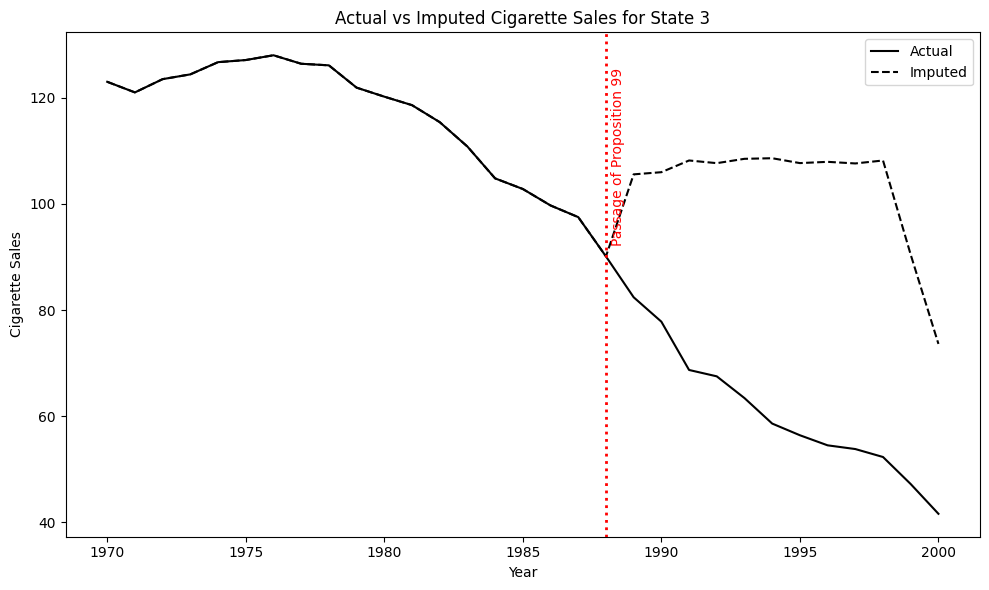
\includegraphics[width=\textwidth]{../figures/cnn-1.png}
        \caption{CNN}
        \label{fig:cnn}
    \end{subfigure}
    \begin{subfigure}[c]{0.45\textwidth}
        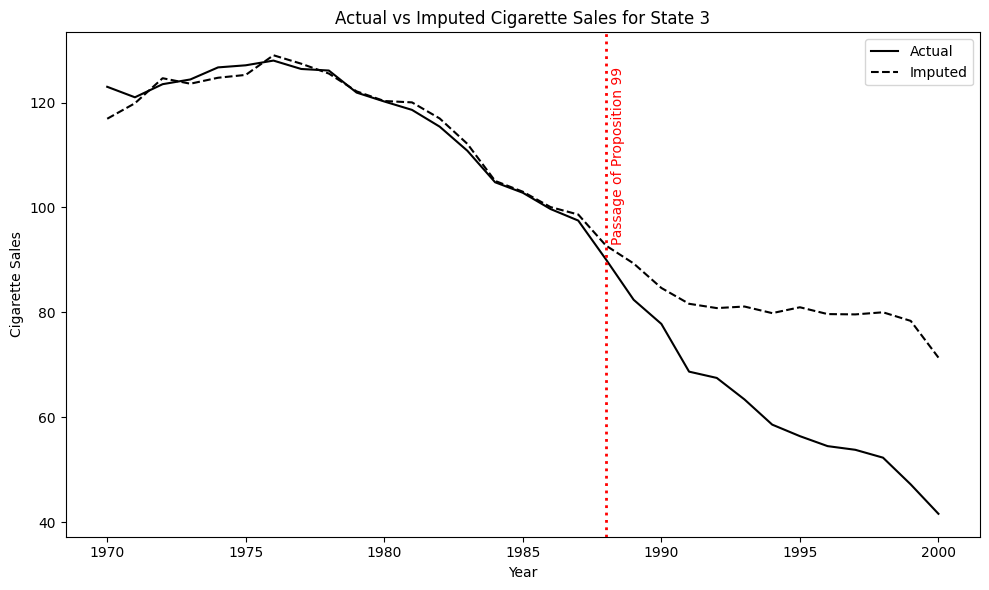
\includegraphics[width=\textwidth]{../figures/mc-nnm-1.png}
        \caption{MC-NNM }
        \label{fig:mcnnm}
    \end{subfigure}
    \caption{Counterfactuals for California Proposition 99 Data}
    \label{fig:main_results}
    \begin{minipage}{0.9\textwidth}
        \scriptsize
        \textbf{Notes:} The left panel shows the CNN counterfactuals, while the right panel shows the MC-NNM counterfactuals for California's cigarette sales data. The horizontal red dashed lines indicate the treatment period. The solid black lines represent the actual outcomes of the treated unit, and the dashed lines represent the predicted counterfactual outcomes.
        In terms of \textcite{rubin1974estimating}'s framework, the gap between the solid and dashed lines represents the estimated treatment effect.
    \end{minipage}
\end{figure}

Figure \ref{fig:main_results} displays the actual and counterfactual outcomes
of California's cigarette sales using CNN and MC-NNM methods.
Subtracting the counterfactuals from the actual outcomes yields the estimated treatment effect of Proposition 99, which is shown as the gap between the solid and dashed lines in Figure \ref{fig:main_results}.
Compared to the MC-NNM results, the CNN counterfactuals were less smooth, and possibly more sensitive to the 
peculiarities of the data.
In terms of direction, both methods produced similar counterfactuals (i.e., both predicted a decrease in cigarette sales after the implementation of Proposition 99),
but the CNN counterfactuals were more volatile, especially in the beginning and the end of the post-treatment periods.

Such sudden surge and drop in the CNN counterfactuals may reflect zero paddings and the convolutional nature of the CNN model,
suggesting that calibration must be done carefully before applying CNNs to panel data.




\subsection{Placebo Tests}

\begin{figure}[htbp]
    \centering
    \begin{subfigure}[c]{0.3\textwidth}
        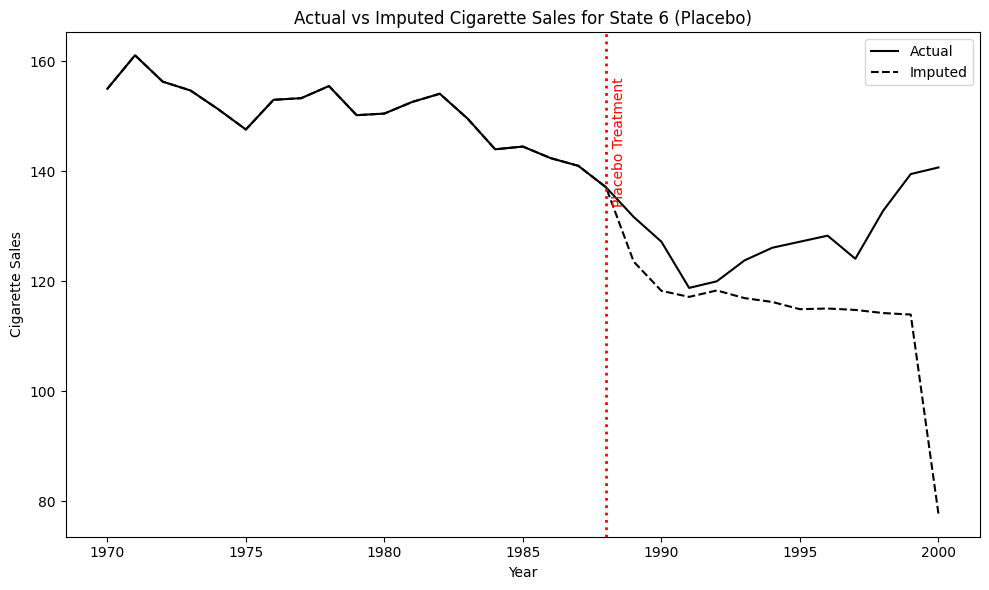
\includegraphics[width=\textwidth]{../figures/cnn-2.png}
        \caption{Delaware}
        \label{fig:placebo_1}
    \end{subfigure}
    \begin{subfigure}[c]{0.3\textwidth}
        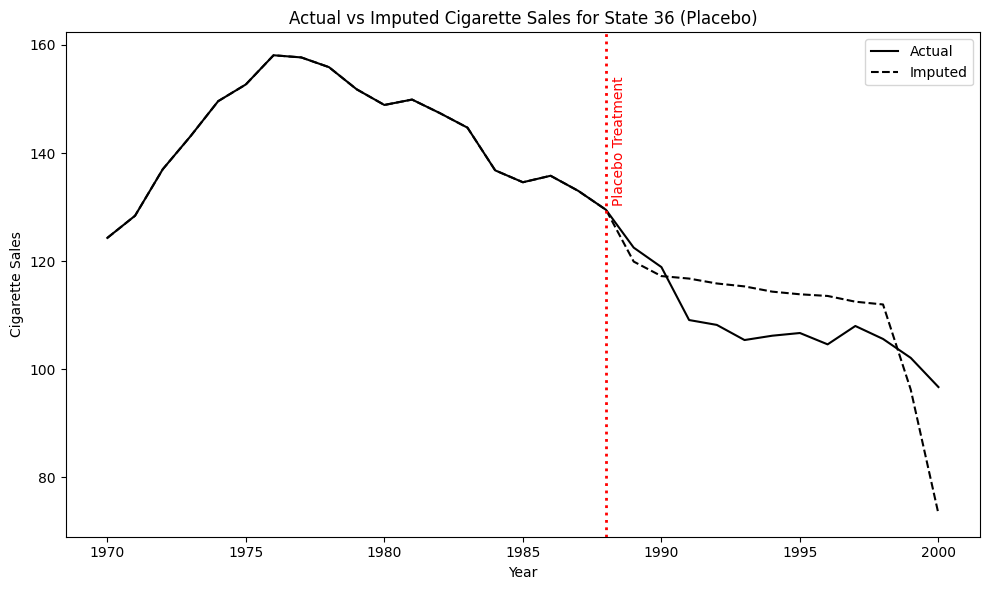
\includegraphics[width=\textwidth]{../figures/cnn-3.png}
        \caption{Virginia}
        \label{fig:placebo_2}
    \end{subfigure}
    \begin{subfigure}[c]{0.3\textwidth}
        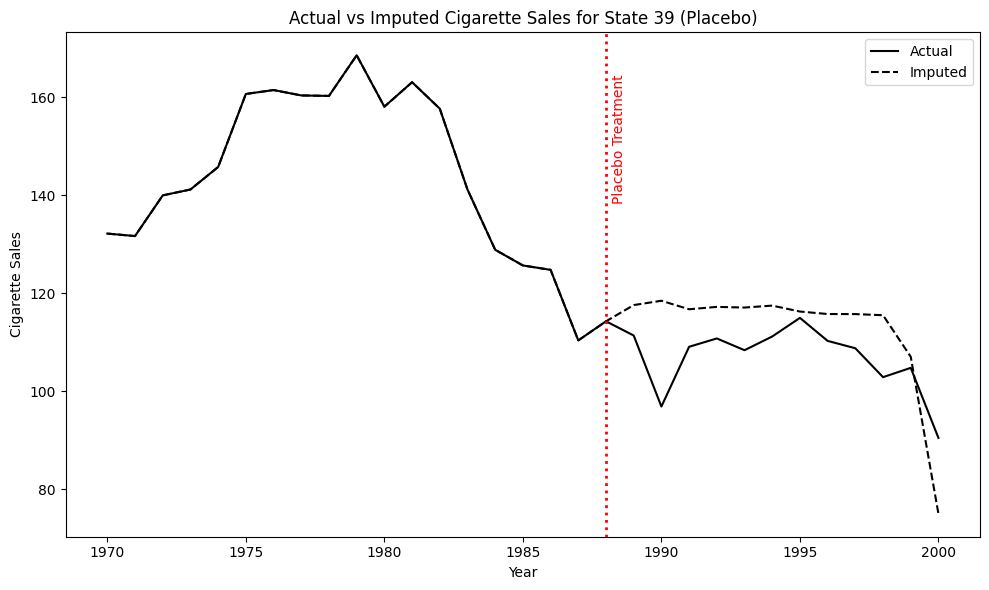
\includegraphics[width=\textwidth]{../figures/cnn-4.png}
        \caption{Wyoming}
        \label{fig:placebo_3}
    \end{subfigure}
    \caption{Placebo Test: CNN Counterfactuals for California Proposition 99 Data}
    \label{fig:placebo_cnn}
\end{figure}


\begin{figure}[htbp]
    \centering
    \begin{subfigure}[c]{0.3\textwidth}
        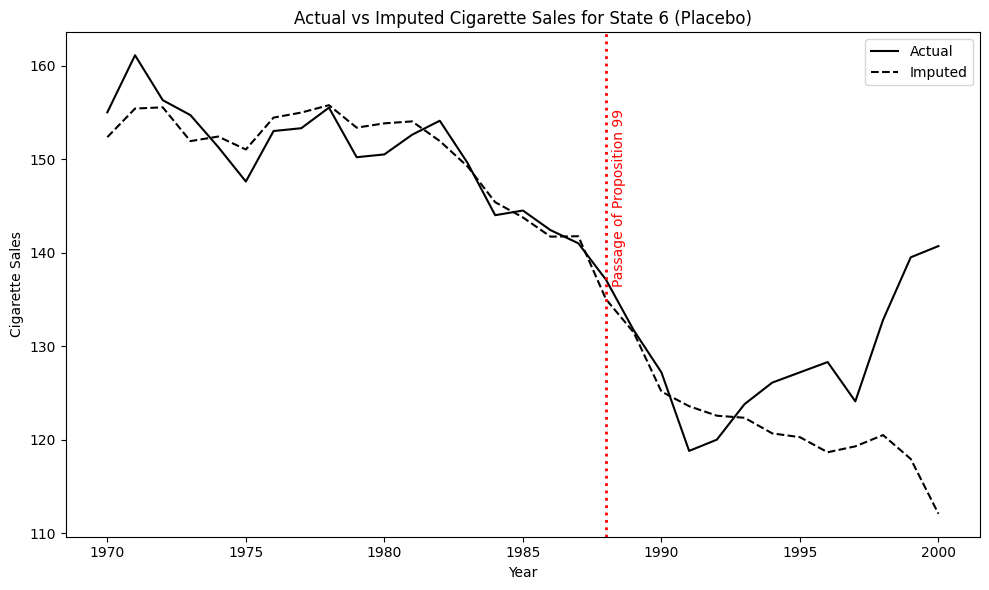
\includegraphics[width=\textwidth]{../figures/mc-nnm-2.png}
        \caption{Delaware}
        \label{fig:placebo_1}
    \end{subfigure}
    \begin{subfigure}[c]{0.3\textwidth}
        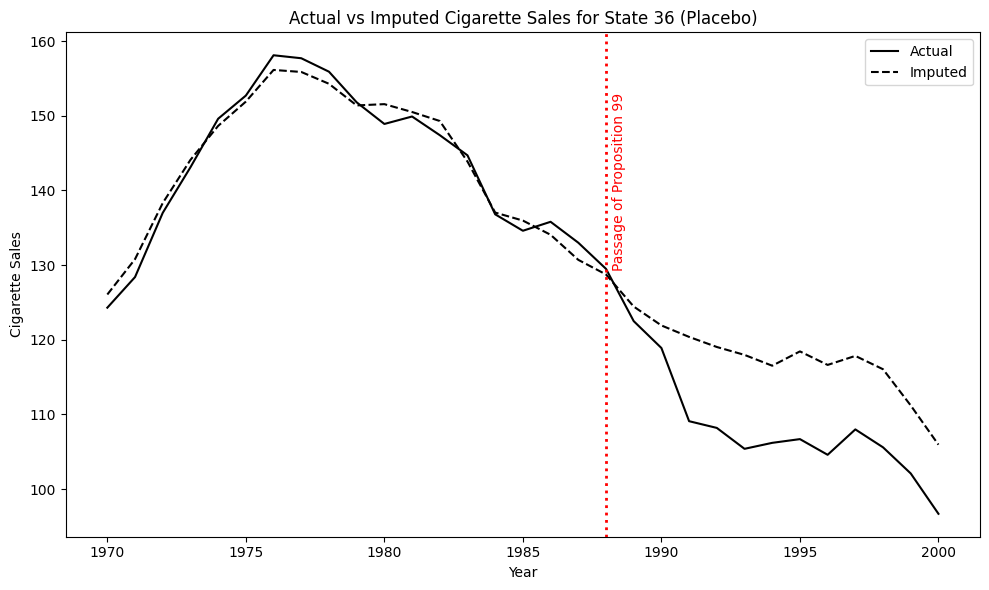
\includegraphics[width=\textwidth]{../figures/mc-nnm-3.png}
        \caption{Virginia}
        \label{fig:placebo_2}
    \end{subfigure}
    \begin{subfigure}[c]{0.3\textwidth}
        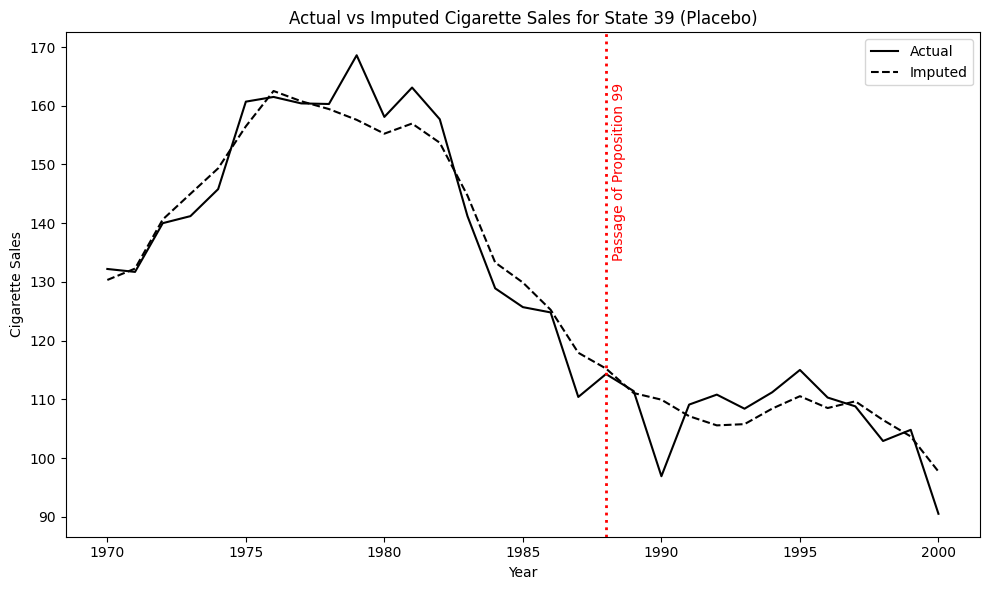
\includegraphics[width=\textwidth]{../figures/mc-nnm-4.png}
        \caption{Wyoming}
        \label{fig:placebo_3}
    \end{subfigure}
    \caption{Placebo Test: MC-NNM Counterfactuals for California Proposition 99 Data}
    \label{fig:placebo_mcnnm}
\end{figure}

To further validate the counterfactual predictions, we conducted placebo tests by applying the CNN and MC-NNM methods to the data, but treating other states as if they were the treated unit and excluding California.
Figures \ref{fig:placebo_cnn} and \ref{fig:placebo_mcnnm} show the results of these placebo tests for CNN and MC-NNM, respectively.


In these figures, we observe that both CNN and MC-NNM methods produce similar predictions for the placebo states and match the actual outcomes closely - reflecting the null treatment effect in these states.
Two patterns are worth noting: first, when MC-NNM does not perform well, CNN fails as well (see Delawre);
second, CNN tends to produce more volatile results at the end of the time series, which reflects the zero padding.


\section{Variations}
In this section, 
we present the results of CNN on California and the three placebo states (Delware, Virginia, and Wyoming)
with two variations in the CNN architecture: (i) applying batch normalization and (ii) adding an additional convolution (with 16 outputs).

\subsection{Batch Normalization}



\begin{figure}[htbp]
    \centering
    \begin{subfigure}[b]{0.4\textwidth}
        \centering
        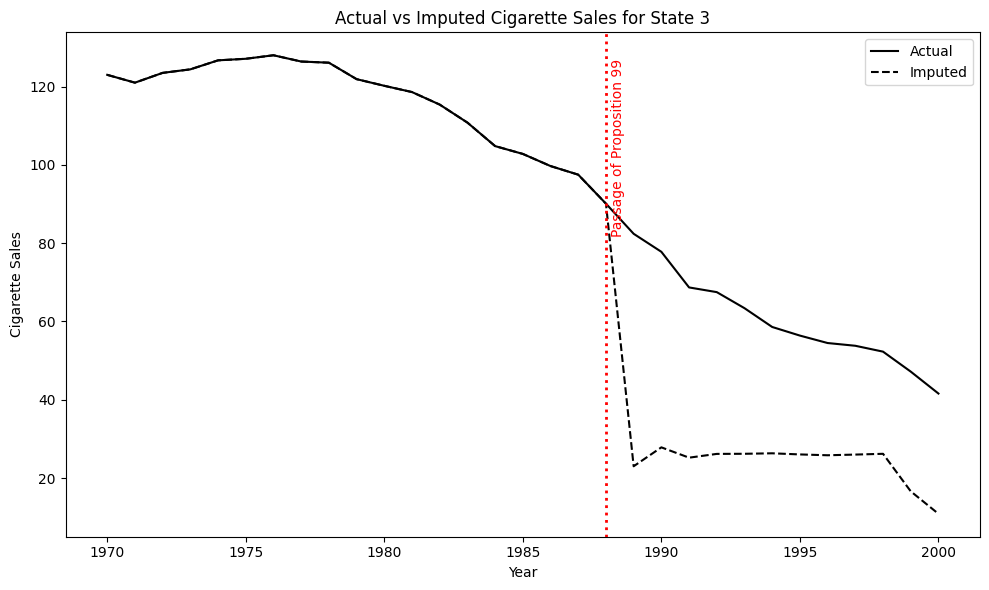
\includegraphics[width=\linewidth]{../figures/cnn_batch_norm-1.png}
        \caption{California}
        \label{fig:bn-cal}
    \end{subfigure}
    \hspace{1.5cm}
    \begin{subfigure}[b]{0.4\textwidth}
        \centering
        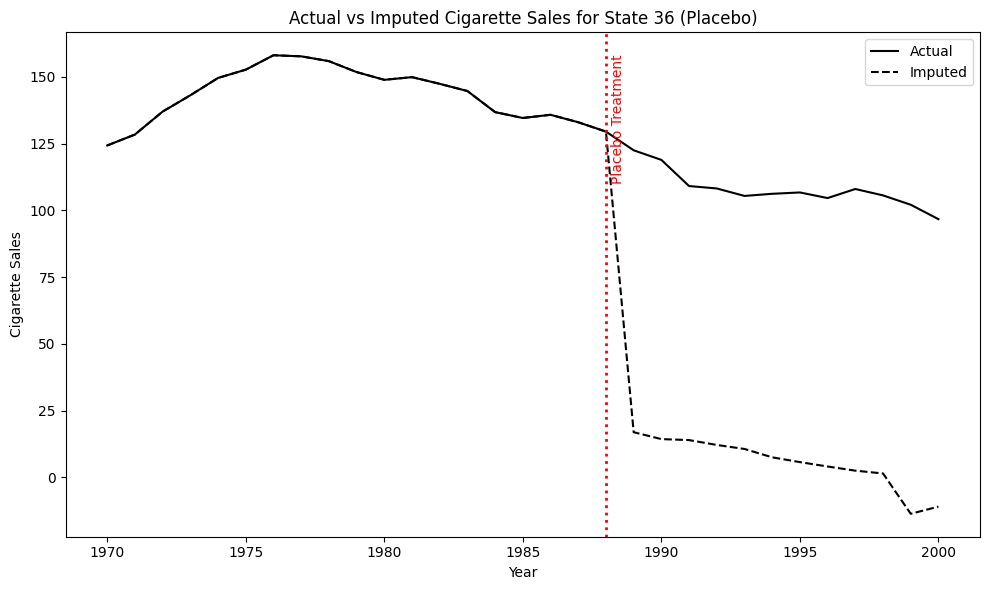
\includegraphics[width=\linewidth]{../figures/cnn_batch_norm-2.png}
        \caption{Delaware}
        \label{fig:bn-del}
    \end{subfigure}

    \vskip\baselineskip

    \begin{subfigure}[b]{0.4\textwidth}
        \centering
        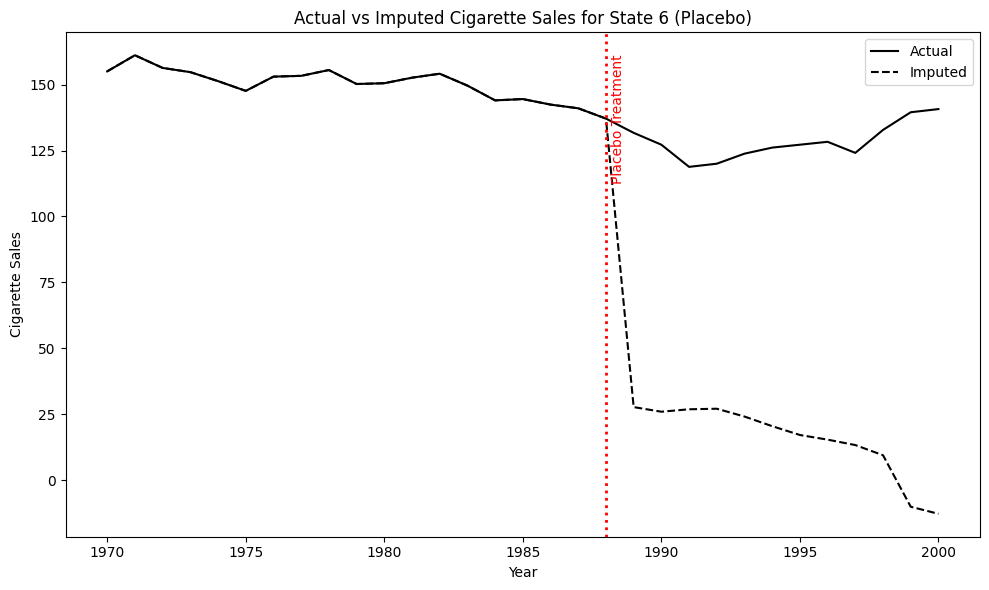
\includegraphics[width=\linewidth]{../figures/cnn_batch_norm-3.png}
        \caption{Virginia}
        \label{fig:bn-vir}
    \end{subfigure}
    \hspace{1.5cm}
    \begin{subfigure}[b]{0.4\textwidth}
        \centering
        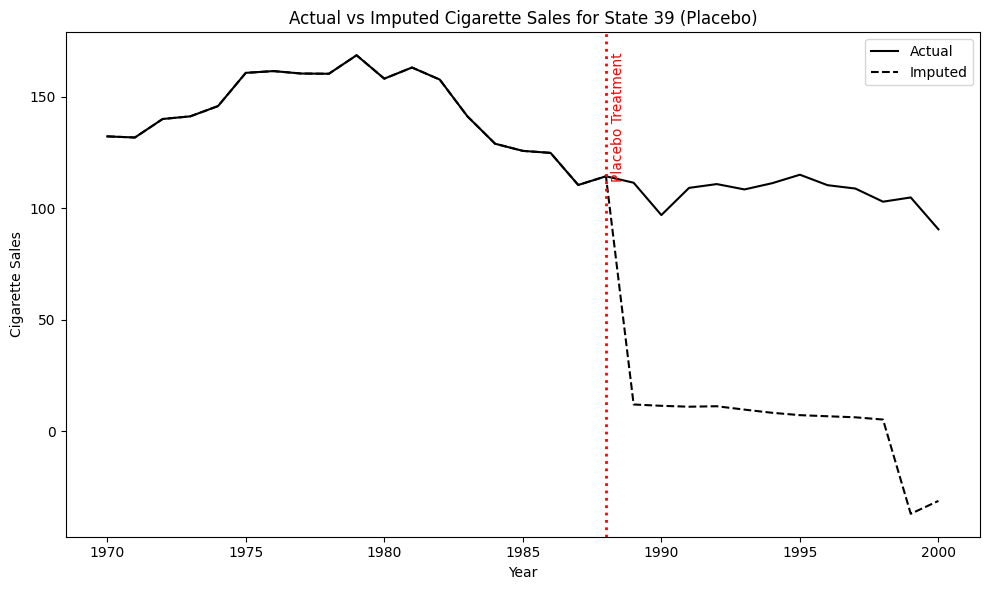
\includegraphics[width=\linewidth]{../figures/cnn_batch_norm-4.png}
        \caption{Wyoming}
        \label{fig:bn-wy}
    \end{subfigure}

    \caption{CNN Counterfactuals with Batch Normalization}
    \label{fig:batch_norm}
\end{figure}

Figure \ref{fig:batch_norm} shows the CNN counterfactuals with batch normalization applied to the California Proposition 99 data.
Panel \ref{fig:bn-cal} shows the counterfactuals for California, the treatment group, and other panels show the counterfactuals for the placebo states (Delaware, Virginia, and Wyoming).

Compared to the original CNN results, the CNN counterfactuals with batch normalization (Figure \ref{fig:batch_norm}) show weaker 
prediction performance. 
Specifically, the counterfactuals plummet after 1989, which is inconsistent in particular with the wide consensus that cigarette sales in California decreased after the implementation of Proposition 99 in 1989.
This suggests that batch normalization may not be suitable for this type of counterfactual prediction task, as the normalization process fits the pre-treatment data too closely, leading to poor generalization to the post-treatment period.


\subsection{Adding Additional Convolutional Layer}

\begin{figure}[htbp]
    \centering
    \begin{subfigure}[b]{0.4\textwidth}
        \centering
        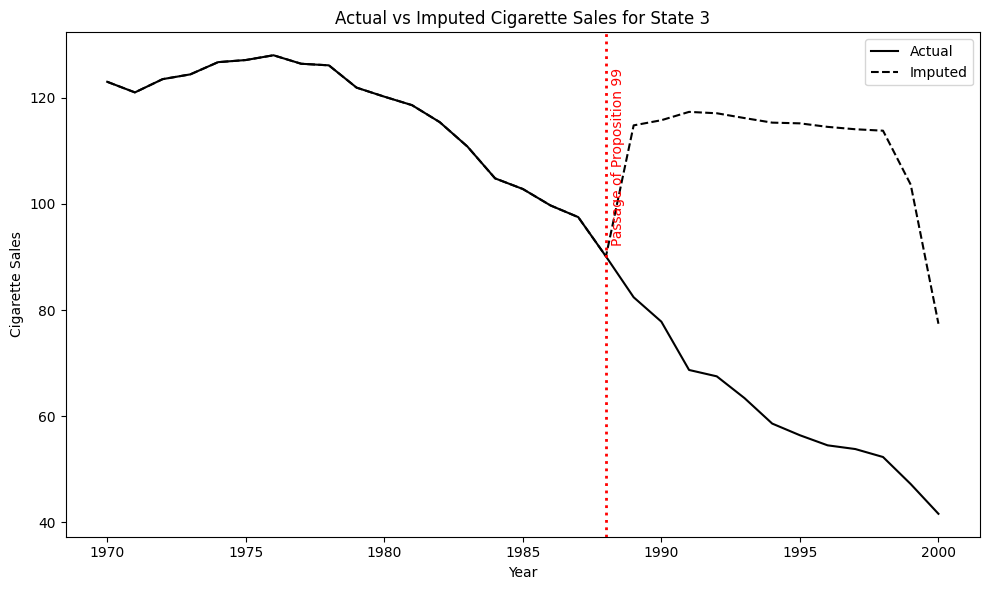
\includegraphics[width=\linewidth]{../figures/cnn_add_layer-1.png}
        \caption{California}
        \label{fig:al-cal}
    \end{subfigure}
    \hspace{1.5cm}
    \begin{subfigure}[b]{0.4\textwidth}
        \centering
        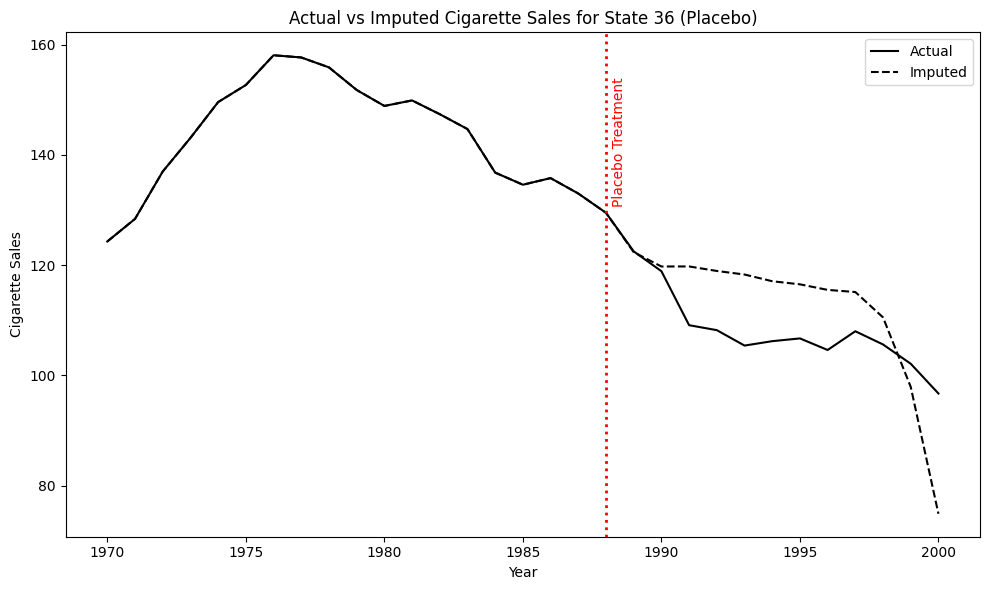
\includegraphics[width=\linewidth]{../figures/cnn_add_layer-2.png}
        \caption{Delaware}
        \label{fig:al-del}
    \end{subfigure}

    \vskip\baselineskip

    \begin{subfigure}[b]{0.4\textwidth}
        \centering
        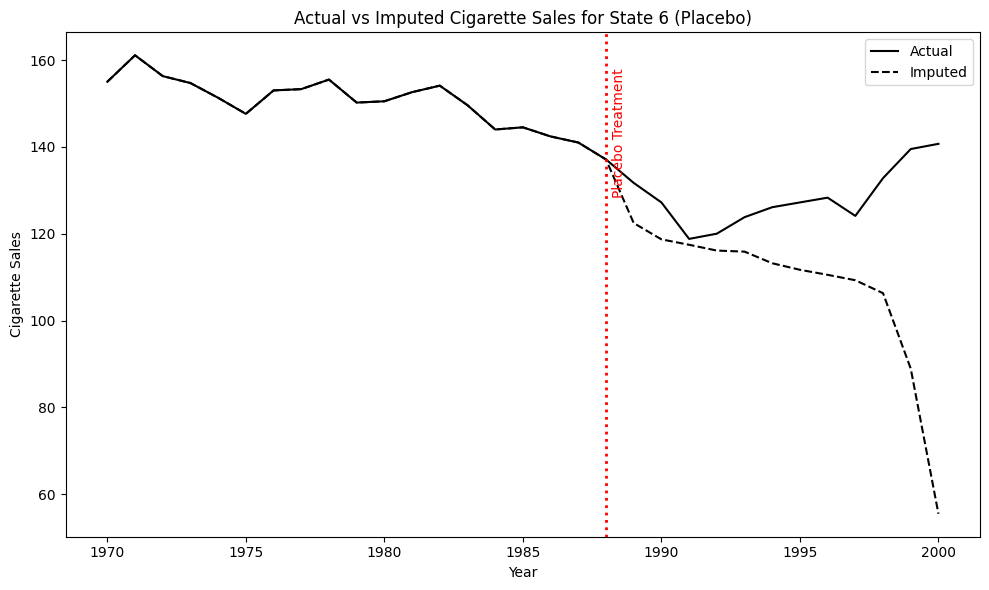
\includegraphics[width=\linewidth]{../figures/cnn_add_layer-3.png}
        \caption{Virginia}
        \label{fig:al-vir}
    \end{subfigure}
    \hspace{1.5cm}
    \begin{subfigure}[b]{0.4\textwidth}
        \centering
        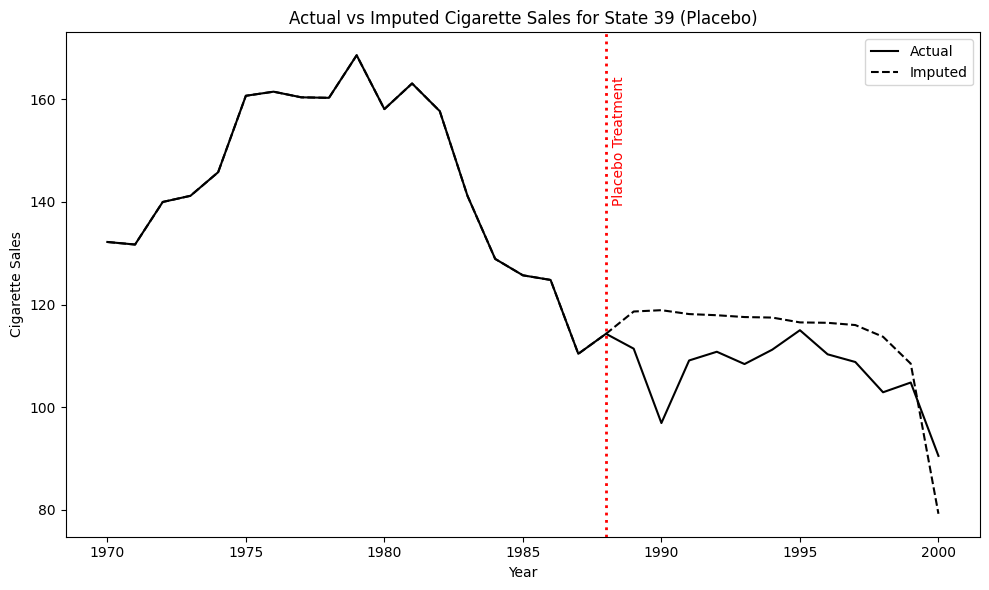
\includegraphics[width=\linewidth]{../figures/cnn_add_layer-4.png}
        \caption{Wyoming}
        \label{fig:al-wy}
    \end{subfigure}

    \caption{CNN Counterfactuals with Additional Layer}
    \label{fig:add_layer}
\end{figure}

Figure \ref{fig:add_layer} shows the CNN counterfactuals with additional convolutional layer with 16 filters and 3$\times 3$ size. applied to the California Proposition 99 data.
Panel \ref{fig:al-cal} shows the counterfactuals for California, the treatment group, and other panels show the counterfactuals for the placebo states (Delaware, Virginia, and Wyoming).

The CNN counterfactuals with additional layer is almost identical to the original CNN results, suggesting that adding an additional convolutional layer does not significantly change the prediction performance.
However, depending on the data size and the complexity of the data generating process, 
adding an additional convolutional layer may improve or worsen the prediction performance in some cases.


\section{Conclusion}

To summarize, this study demonstrates the potential of applying convolutional neural networks (CNNs) to panel data analysis, particularly in the context of causal inference.
However, potential issues such as overfitting and sensitivity to data peculiarities must be addressed, including
the poor prediction performance on the final period.
Future research should focus on refining the CNN architecture and exploring alternative methods to improve the robustness of counterfactual predictions.
For example, considering the autoregressive nature of panel data, incorporating PixelCNN or BiLSTM that 
can capture temporal dependencies may enhance the model's performance.
Additionally, further validation through extensive simulations and real-world applications is necessary to establish the reliability and generalizability of CNNs in causal panel data models.

\newpage
\printbibliography

\end{document}